
\textbf{\underline{Во первой главе}} показан обзор существующих решений. Рассмотрены 3 глобальных темы: типы препятствий, которые могут встретиться; роботы, которые используются в исследованиях пещер; а так же методы построения карты местности.

Была проведена классификация машин, использующих ноги в качестве движителя. Подводя итог, можно сказать, что классификация следующая. Важно отметить, что в одном экземпляре может сочетаться несколько типов движителей.
\begin{enumerate}
    \item Псевдошагающие машины
    \item Шагающие машины с дополнительными опорными механизмами
    \item Шагающие машины с движителями циклического действия
    \item Ходьба с импровизированным следом
    \begin{enumerate}
    \item Ходьба - колесная
    \item Прыжки и бег
    \item Ползание
    \item Лазание
    \end{enumerate}
    \end{enumerate}
    
В диссертации рассматривались роботы которые создавались специально для исследований пещер, в том числе и на Марсе. А так же те, которые потенциально могут быть использованы в условиях, определенных выше.

Как итог, их можно классифицировать следующим образом. Наземные роботы это шагающие, колесные, трековые и необычные. К необычным включены змеевидные, шарообразные и другие. К летающим были отнесены защищенные дроны и дирижабли.

Полноценной робототехнической системой является система, включающая в себя несколько роботов одного типа или комбинацию наземного и летающего роботов.

Для решения поставленной цели необходимо понимать в каких условиях будет использоваться робот. Основные структуры поверхностей следующие \pic{fig:obstacles}:
\begin{itemize}
    \item твердые породы, прочные -- мрамор, кварц, базальт (магма);
    \item твердые породы, мягкие -- мел, гипс, соль, известняк;
    \item сыпучие грунты -- песок, глина, снег;
    \item водные преграды -- как и лужи (малый слой воды), так и целы залы, погруженные под воду. Часто встречаются сифоны;
    \item скользкие поверхности -- отложения мха и плесени, лед ;
    \item разрушаемые поверхности -- каменная гряда, паутина.
\end{itemize}



Так же были рассмотрены размеры пещер, чтобы понимать необходимый запас хода, размеры робототехнического комплекса.

Были рассмотрены классические SLAM алгоритмы, основанные на использовании камеры, стереопары, с использованием лидара, GPS, IMU а так же их различные комбинации. 

Проведен обзор триангуляций, так как данный метод лежит в основе определения геометрических свойств объекта.

Были найдены способы получения облака точек объекта с помощью касания манипулятором данного объекта. Примерное местоположение объекта определялось камерой.

Определить тип поверхности можно так же с помощью различных сенсоров: визуально, IMU, с помощью снятия тока с моторов, момента с вала мотора, с помощью датчиков силы, установленных на конечность робота.

Были найдены следующие предложенные решения:
\begin{itemize}
    \item робототехнические системы для исследования свободных пещер;
    \item Построение карты с помощью лидаров и камер;
    \item Получение конечно элементной сетки с помощью тактильного очувствления манипулятором.
\end{itemize}

Поставленная задача является новой и не встречается в научных публикациях российских и зарубежных авторов.

Итогом первой главы является создание обзора разработанной системы \pic{fig:diag_system.png}.
\begin{figure}[H]
    \centering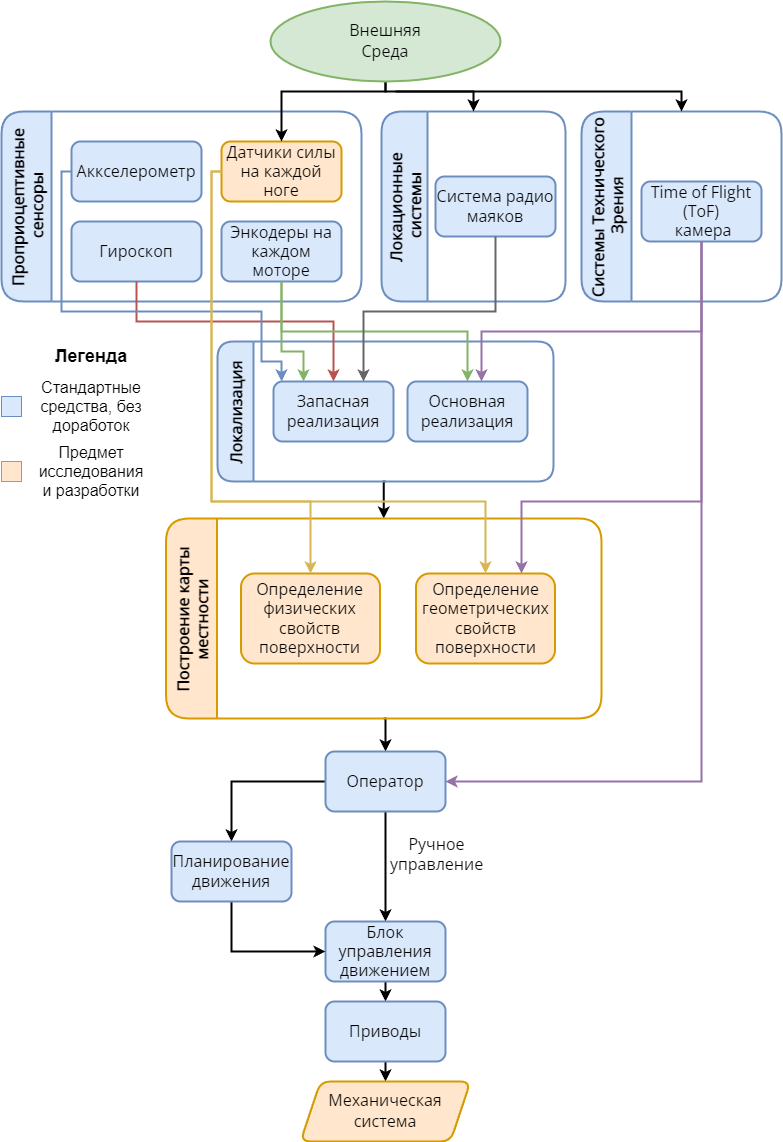
\includegraphics[height=16cm,width=1\textwidth,keepaspectratio]{main_diag.drawio.png}
    \caption{Структурная схема разработанной системы}
    \label{fig:diag_system.png}
\end{figure}

Оранжевым цветом выделены те компоненты системы, которые представляют собой предмет исследования в рамках диссертационной работы. Их разработка и научная новизна описаны в последующих главах диссертации. Голубым цветом выделены блоки, соответствующие которым элементы в разработанную систему были интегрированы как стандартные средства,   без каких-либо существенных доработок.

Верхний блок --- внешняя среда, то есть вся информация о внешнем мире, с которой работает робот.

Следующая группа блоков связана с сенсорами. Здесь представлены <<Проприоцептивные сенсоры>>, то есть внутренние датчики, такие как гироскоп, акселерометр, энкодеры и датчики силы. Также есть группа блоков, посвященная техническому зрению. Последней группой элементов является <<Локационные системы>>, представленные системой радио маяков. 

Ниже находится следующая группа блоков <<Локализация>>. Она основана на данных, полученных с сенсоров. В данной группе расположены два блока <<Основная реализация>> и <<Запасная реализация>>. Первая является более точной. Она может быть реализована на основе системы радио маяков или с помощью системы технического зрения. Но самый точный результат может быть получен при объединении двух систем. Запасная реализация является резервной, когда отказала основная реализация, или когда та выдает некорректные результаты. Она основана на Инерциальном измерительном устройстве (IMU), датчиках силы и системе маяков.

В рамках диссертационного исследования были разработаны следующая группа блоков <<Построение модели местности>> был реализован и разработан автором диссертации. Она состоит из трех блоков: <<Определение физических свойств поверхности>>, <<Построение карты местности>>, <<Определение геометрических свойств поверхности>>. Первый блок позволяет параллельно с исследованием геометрических свойств поверхности, посредством ее пальпирования, определять материал по которому ходит робот. Построение карты местности объединяет данные с других двух блоков и выводит результат в машино и человеко читабельные виды. Более подробно данная группа описана в главе \nameref{ch:ch4}.

Полученные данные попадают оператору, и оператор может управлять роботом, как в ручном режиме, так и просто задав область, куда роботу нужно прийти. Эта высокоуровневая команда передается в блок управления движением, которая в последствии преобразуется в низкоуровневые команды для приводов робота. С помощью данных команд, механическая система, представленная разработанным роботом приводится в движение и выполняется поставленная оператором задача.

В работе научная новизна представлена в элементах схемы, связанных с очувствлением: датчики силы, построение карты местности, определение физических свойств объекта.
